\section{Mediciones}

Se realizaron mediciones en base a crear pruebas de distintos tamaños y tomar su tiempo de ejecución individualmente, y en base a los datos recolectados hacer el gráfico. Los datos fueron desde 10000 hasta 100000 elementos, los cuales los tiempos tanto de Scaloni como los ayudantes para cada uno de los rivales fue un número aleatorio desde 1000 hasta 10000.

\begin{figure}[H]
	\centering
	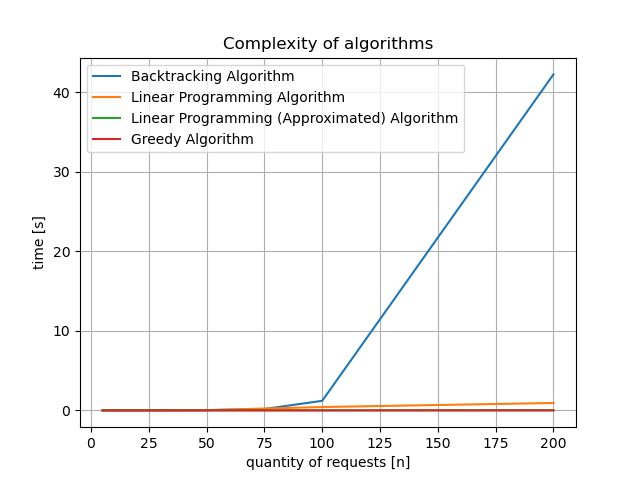
\includegraphics[width=1\textwidth]{img/graphic.png}
\end{figure}

Como se puede apreciar, el algoritmo Greedy efectivamente fue veloz, tal como se los suele caracterizar. A su vez, se puede ver que se asemeja a la complejidad indicada, ya que la tendencia es aproximadamente lineal en términos de $\mathcal{O}\left(n \log n\right)$.
